\documentclass{beamer}
\usepackage[utf8]{inputenc}
\usetheme{Madrid}
\usecolortheme{default}
\setbeamertemplate{navigation symbols}{}

\usepackage{hyperref}

\usepackage{tikz}
\usetikzlibrary{calc}
\usetikzlibrary{intersections}

\usepackage{graphicx}
\graphicspath{ {./graphics/} }

\usepackage{float}

\title[Orthonormal Basis]{Orthonormal Basis, Gram-Schmidt Process ($\mathbb{R}^n$)}
\author{Pascal Pilz}
\institute{KO Mathematics for AI II}
\date{\today}

\AtBeginSection[]
{
  \begin{frame}
    \frametitle{Table of Contents}
    \tableofcontents[currentsection]
  \end{frame}
}

\makeatletter
\setbeamertemplate{headline}{%
    \begin{beamercolorbox}[ht=2.25ex,dp=3.75ex]{section in head/foot}
        \insertnavigation{\paperwidth}
    \end{beamercolorbox}%
}%
\makeatother

%=========================================================
\begin{document}

%---------------------------------------------------------
\frame{\titlepage}

%---------------------------------------------------------
\begin{frame}
    \frametitle{Table of Contents}
    \tableofcontents
\end{frame}


%=========================================================
\section{Recap Vector space, Span, Basis; Definition Orthogonal, Orthonormal Basis}

%---------------------------------------------------------
\begin{frame}
    \small
    \begin{block}{Definition (Vector space)}
        By a \textbf{vector space} we shall mean a set $V$ on which there are defined two operations, one called "addition" and the other called "multiplication by scalars", such that the following properties hold:
        \begin{align*}
            &(V_1) \quad x+y = y+x \text{ for all } x,y \in V;\\
            &(V_2) \quad (x+y)+z = x+(y+z) \text{ for all } x,y,z \in V;\\
            &(V_3) \quad \text{there exists an element } 0 \in V \text{ such that } x+0 = x \text{ for every } x \in V;\\
            &(V_4) \quad \text{ for every } x \in V \text{ there exists } -x \in V \text{ such that } x+(-x) = 0;\\
            &(V_5) \quad \lambda (x+y) = \lambda x + \lambda y \text{ for all } x,y \in V \text{ and all scalars } \lambda;\\
            &(V_6) \quad ( \lambda + \mu ) x = \lambda x + \mu x \text{ for all } x \in V \text{ and all scalars } \lambda, \mu;\\
            &(V_7) \quad (\lambda \mu) x = \lambda ( \mu x) \text{ for all } x \in V \text{ and all scalars } \lambda, \mu;\\
            &(V_8) \quad 1x = x \text{ for all } x \in V. 
        \end{align*}
        
        When the scalars are all real numbers we shall often talk of a \textbf{real} vector space;  when the scalars are all complex numbers we shall talk of a \textbf{complex} vector space.
        
        \par \vspace{1mm} (Basic Linear Algebra, Blyth, T.S. and Robertson, E.F., 2002, p. 69)
    \end{block}
\end{frame}

%---------------------------------------------------------
\begin{frame}{Inner product}
    \small
    \begin{block}{Definition (Inner product)}
        Let $V$ be a vector space over $\mathbb{C}$. By an \textbf{inner product} on $V$ we shall mean a mapping $f: V \times V \to \mathbb{C}$, described by $(x,y) \mapsto \langle x | y \rangle$, such that for all $x, x', y \in V$ and for all $\alpha \in \mathbb{C}$, the following identities hold:
        \begin{align*}
            &(1) \quad \langle x + x' | y \rangle = \langle x | y \rangle + \langle x' | y \rangle;\\ 
            &(2) \quad \langle \alpha x | y \rangle = \alpha \langle x | y \rangle;\\
            &(3) \quad \overline{\langle x | y \rangle} = \langle y | x \rangle \text{ so that in particular } \langle x | x \rangle \in \mathbb{R};\\
            &(4) \quad \langle x | x \rangle \geq 0, \text{ with euqality if and only if } x = 0_V.
        \end{align*}
        
        By a \textbf{complex inner product space} we mean a vector space $V$ over $\mathbb{C}$ together with an inner product on $V$. By a \textbf{real inner product space} we mean a vector space $V$ over $\mathbb{R}$ together with an inner product on $V$.
        
        \par \vspace{3mm} (Further Linear Algebra, Blyth, T.S. and Robertson, E.F., 2002, p. 11)
    \end{block}
\end{frame}

%---------------------------------------------------------
\begin{frame}{Example Inner product}
    \small
    \begin{example}
        On the vector space $\mathbb{R}^n$ of $n$-tuples of real numbers let
        $$\langle (x_1, \dots, x_n) | (y_1, \dots, y_n) \rangle = \sum_{i=1}^{n}{x_i y_i}.$$
        Then it is readily verified that this defines an inner product on $\mathbb{R}^n$, called the \textbf{standard inner product} on $\mathbb{R}^n$.\\
        In the cases where $n = 2,3$ this inner product is often called the \textbf{dot product} or \textbf{scalar product}. This terminology is popular when dealing with the geometric applications of vectors. Indeed, several of the reults that we shall establish will generalise familiar results in euclidian geometry of two and three dimesnions.

        \par \vspace{3mm} (Further Linear Algebra, Blyth, T.S. and Robertson, E.F., 2002, p. 12, Example 1.1)
    \end{example}
\end{frame}

%---------------------------------------------------------
\begin{frame}{Span}
    \begin{block}{Definition (Span)}
        Let $V$ be a vector space over a field $F$ and let $S$ be a non-empty subset of $V$. Then we say $v \in V$ is a \textbf{linear combination of elements of $S$} if there exists $x_1, \dots, x_n \in S$ and $\lambda_1, \dots , \lambda_n \in F$ such that
        $$v = \lambda_1 x_1 + \dots + \lambda_n x_n = \sum_{i=1}^{n} \lambda_i x_i.$$
        
        It is clear that if $v = \sum_{i=1}^{n} \lambda_i x_i$ and $w = \sum_{i=1}^{n} \mu_i y_i$ are linear combination of elements of $S$ then so is $v + w$; moreover, so is $\lambda v$ for every $\lambda \in F$. Thus the set of linear combinations of elements of $S$ is a subspace of $V$. We call this the \textbf{subspace spanned by $S$} and denote it by \alert{Span $S$}.

        \par \vspace{3mm} (Basic Linear Algebra, Blyth, T.S. and Robertson, E.F., 2002, p. 75-76)
    \end{block}
\end{frame}

%---------------------------------------------------------
\begin{frame}{Example Span I}
    \begin{example}
        Consider the subset $S_1 = \{\alert{(1,0)}, \alert{(0,1)}\}$ of the cartesian plane $\mathbb{R}^2$. For every $(x,y) \in \mathbb{R}^2$ we have
        $$(x,y) = (x,0) + (0,y) = x\alert{(1,0)} + y\alert{(0,1)},$$
        so that every element of $\mathbb{R}^2$ is a linear combination of elements of $S_1$. Thus $S_1$ is a spanning set of $\mathbb{R}^2$.
        \par \vspace{3mm} (Basic Linear Algebra, Blyth, T.S. and Robertson, E.F., 2002, p. 76, Example 5.14)
    \end{example}
\end{frame}

%---------------------------------------------------------
\begin{frame}{Example Span II}
    \begin{example}
        Consider the subset $S_2 = \{\alert{(1,2)}, \alert{(-1,-1/2)}\}$ of the cartesian plane $\mathbb{R}^2$. For every $(x,y) \in \mathbb{R}^2$ we have
        $$(x,y) = \frac 1 3 (2y - x) \cdot \alert{(1,2)} + \frac 2 3 (y - 2x) \cdot \alert{(-1, -1/2)},$$
        so that every element of $\mathbb{R}^2$ is a linear combination of elements of $S_2$. Thus $S_2$ is a spanning set of $\mathbb{R}^2$.
    \end{example}
\end{frame}

%---------------------------------------------------------
\begin{frame}{Linearly independent}
    \begin{block}{Definition (Linearly independent)}
        Let $S$ be a non-empty subset of a vector space $V$ over a field $F$. Then $S$ is said to be \textbf{linearly independent} if the only way of expressing $0_V$ as a linear combination of elements of $S$ is the trivial way (in which all scalars are $0_F$.
        Equivalently, $S$ is linearly independent if, for any given $x_1, \dots, x_n \in S$, we have
        $$\lambda_1 x_1 + \dots \lambda_n x_n =0_V \quad \Rightarrow \quad \lambda_1 = \dots = \lambda_n = 0_F.$$
        \par \vspace{3mm} (Basic Linear Algebra, Blyth, T.S. and Robertson, E.F., 2002, p. 78)
    \end{block}
\end{frame}

%---------------------------------------------------------
\begin{frame}{Linear Independence, Basis}
    \begin{theorem}[Linear independence, linear combination]
        Let $V$ be a vector space over a field $F$. If $S$ is a subset of $V$ that contains at least two elements then the following statements are equivalent:
        \begin{itemize}
        	\item $S$ is linearly dependent;
        	\item at least one element of $S$ can be expressed as a linear combination of the other elements of $S$.
        \end{itemize}
        \par \vspace{1mm} (Basic Linear Algebra, Blyth, T.S. and Robertson, E.F., 2002, p. 78, Theorem 5.5)
    \end{theorem}
    
    \pause
    
    \begin{block}{Definition (Basis)}
        A \textbf{basis} of a vector space $V$ is a \textbf{linearly independent} subset of $V$ that \textbf{spans} $V$.
        \par \vspace{1mm} (Basic Linear Algebra, Blyth, T.S. and Robertson, E.F., 2002, p. 80)
    \end{block}
\end{frame}

%---------------------------------------------------------
\begin{frame}{Orthogonal, Orthonormal, Orthonormal Basis}
    \tiny
    In the following we mean by $\| x \| = \sqrt{\langle x | x \rangle}$. For more detail see \emph{Further Linear Algebra, Blyth, T.S. and Robertson, E.F., 2002, p. 11}.
    \normalsize
    
    \pause
    
    \begin{block}{Definition (Orthogonal, orthonormal)}
        If $V$ is an inner product space then $x,y \in V$ are said to be \textbf{orthogonal} if $\langle x | y \rangle = 0$. A non-empty subset $S$ of $V$ is said to be an \textbf{orthogonal subset} if every pair of distinct elements of $S$ is orthogonal. An \textbf{orthonormal subset} of $V$ is an orthogonal subset $S$ such that $\| x \| = 1$ for every $x \in S$.
        \par \vspace{1mm} (Further Linear Algebra, Blyth, T.S. and Robertson, E.F., 2002, p. 17)
    \end{block}
    
    \pause
    
    \begin{block}{Definition (Orthonormal basis)}
        By an \textbf{orthonormal basis} of a inner product space we mean an orthonormal subset that is a basis.
        \par \vspace{1mm} (Further Linear Algebra, Blyth, T.S. and Robertson, E.F., 2002, p. 17)
    \end{block}
\end{frame}

%---------------------------------------------------------
\begin{frame}{Examples Orthonormal Basis}
    \begin{example}[I]
        The standard bases of $\mathbb{R}^n$ and of $\mathbb{C}^n$ are orthonormal bases.\par
        I.e., for $\mathbb{R}^n$ we have ${e_1, \dots, e_n}$ with $e_i = (\underbrace{0, \dots, 0}_{i-1}, 1, 0,  \dots, 0)$.
        \par \vspace{1mm} (Further Linear Algebra, Blyth, T.S. and Robertson, E.F., 2002, p. 16, Example 1.10)
    \end{example}
    
    \pause
    
    \begin{example}[II]
        In $Mat_{n \times n}\mathbb{C}$ with $\langle A | B \rangle = \sum_{i=1}^{n}c_{ii}$ for $[c_{ij}]_{n \times n} = B\!*\!A$ an orthonormal basis is $\{E_{p,q} ; p, q = 1, \cdots, n\}$ where $E_{p,q}$ has a $1$ in the $(p,q)$-th position and $0$ elsewhere.
        \par \vspace{3mm} (Further Linear Algebra, Blyth, T.S. and Robertson, E.F., 2002, p. 18, Example 1.11)
    \end{example}
\end{frame}

%=========================================================
\section[Gram-Schmidt Process]{Gram-Schmidt Process for orthonormalizing a set of vectors}

%---------------------------------------------------------
\begin{frame}{Gram-Schmidt orthonormalization process, what is it good for?}
    We \textbf{take a set of vectors $X$ that spans a vector space} $V$, i.e., is a basis of $V$, and \textbf{return another set of vector $Y$ that spans the same space}. The set $Y$ is orthonormal.\par
    Consider for example the vector space $\mathbb{R}^2$, the cartesian plane. Vectors can here commonly be represented as arrows, starting at the origin $(0,0)$ and ending up at the point they describe $(x_1, x_2)$. The commonplace basis for this space are the two unit vectors $e_1 = (1,0)$ and $e_2 = (0,1)$. Nevertheless this space can actually be spanned by any two linearly independent vectors. That is, any two vectors that do not point in the same direction can act as a basis for this space.
\end{frame}

%---------------------------------------------------------
\begin{frame}{Gram-Schmidt orthonormalization process}
    \small
    \begin{theorem}[Gram-Schmidt orthonormalization process]
        Let $V$ be an inner product space and for every non-zero $x \in V$ let $x^* = x / \| x \|$. If $\{x_1 , \dots , x_k\}$ is a linearly independent subset of $V$, define recursively
        \begin{align*}
            y_1 &= x_1^*;\\
            y_2 &= \left( x_2 - \langle x_2 | y_1 \rangle y_1 \right)^*;\\
            y_3 &= \left( x_3 - \langle x_3 | y_2 \rangle y_2 - \langle x_3 | y_1 \rangle y_1 \right)^*;\\
            &\vdots \\
            y_k &= \Bigl( x_k - \sum_{i=1}^{k-1} \langle x_k | y_i \rangle y_i \Bigl)^*.
        \end{align*}

        Then $\{y_1, \dots, k_k\}$ is orthonormal and spans the same subspace as $\{x_1, \dots, x_k\}$.

        \par \vspace{2mm} (Further Linear Algebra, Blyth, T.S. and Robertson, E.F., 2002, p. 18, Th. 1.4)
    \end{theorem}
\end{frame}

%---------------------------------------------------------
\begin{frame}{Gram-Schmidt process in words}
    In words, using the intuitive notion of arrows on vectors in $\mathbb{R}^2$:\par
    A (random) first vector $x_1$ gets normalized to length 1, the normalized vector is $y_1$. A next vector $x_2$ gets chosen, from this vector, we subtract the part of its direction pointing towards the first vector by getting the inner product $\langle y_1 | x_2 \rangle$, which so-to-say gives the length of the projection of $x_2$ onto $y_1$, now we multiply this scalar we got from the inner product with the direction of $y_1$ and subtract this value form $x_2$. This leaves us with only the part of the direction pointing perpendicular to the first vector. This part now gets normalized to length 1 and becomes $y_2$.\par
    The process continues like this, taking into consideration all previously established vectors.
\end{frame}

%---------------------------------------------------------
\begin{frame}{Gram-Schmidt process visualization}
    \begin{columns}
        \column{0.5\textwidth}
            \begin{center}
                \begin{tikzpicture}[scale=1.5]
                    \coordinate (x1) at (70:2.1cm);
                    \coordinate (x2) at (13:1.4cm);
                    \coordinate (0) at (0,0);
                    
                    \draw[step=1, gray, very thin] (-1.5,-1.5) grid (2.5,2.5);
                    \draw[->, very thick] (0) -- (2.5,0);
                    \draw[->, very thick](0)-- (0,2.5);
                    \draw[->, very thick](0)-- (0,-1.5);
                    \draw[->, very thick](0)-- (-1.5,0);
                    \draw (2pt, 1) -- (-2pt, 1) node[left]{1};
                    \draw (1, 2pt) -- (1, -2pt) node[below]{1};

                    \draw<3-5> [gray] ($(0)!(x2)!(x1)$) -- (x2);
                    \draw<3-5>[gray] ($($(0)!(x2)!(x1)$)+({0.1*cos(-18)},{0.1*sin(-18)})$) arc (-18:72:0.1);
                    \node<3-5>[gray] at (0.31cm, 0.738cm) {.};
                    \draw<5->[gray] ($(0)+({0.2*cos(-18)},{0.2*sin(-18)})$) arc (-18:72:0.2);
                    \node<5->[gray] at (0.1cm, 0.05cm) {.};
                    % Don't judge me for how i hard coded these shapes ;-;. I don't want to spend any more time trying to construct this dot or the arc properly
        
                    \draw<1>[->, red, thick](0)--(x1)node[above]{$x_1$};
                    %\path[name path=x1path](0)-- x1;
                    \draw<1>[->, blue, thick](0)--(x2)node[right]{$x_2$};
                    %\path[name path=x2](0)-- x2;
                    
                    \draw<2->[->, red, opacity=0.3](0)--(x1)node[above]{$x_1$};
                    \draw<2->[->, blue, opacity=0.3](0)--(x2)node[right]{$x_2$};
                    
                    \draw<2->[->, magenta, thick](0)-- (70:1cm) node[right]{$y_1$};
                    
                    \draw<3-5> [green, thick] ($(0)!(x2)!(x1)$) -- 0;

                    \draw<4-5> [->, green, thick] (x2) -- ($(x2) - ($(0)!(x2)!(x1)$)$);
                    \draw<5> [->, cyan, thick] (0) -- ($(x2) - ($(0)!(x2)!(x1)$)$);

                    \coordinate (b) at ($(0)!(x2)!(x1)$);
                    \coordinate (a) at ($(x2) - (b)$);
                    \draw<6> [->, green, opacity=0.3] (x2) -- ($(x2) - ($(0)!(x2)!(x1)$)$);
                    \draw<6> [->, cyan, opacity=0.3] (0) -- ($(x2) - ($(0)!(x2)!(x1)$)$);
                    \draw<6> [->, cyan, thick] (0) -- ($(0)!1cm!(a)$) node[below] {$y_2$};
                \end{tikzpicture}
            \end{center}
        \column{0.5\textwidth}
            \begin{enumerate}
                \item<2-> Normalize $x_1$ to get $y_1$
                \item<3-> Green is $x_2$ projected onto $y_1$, aka $\langle x_2 | y_1 \rangle y_1$
                \item<4-> Subtract green from $x_2$
                \item<5-> What you get is a vector perpendicular to $y_1$. Now normalize this vector to length 1
                \item<6-> The result is $y_2$. $y_2$ is perpendicular to $y_1$ and has a length of 1, i.e., $\langle y_1 | y_2 \rangle = 0$ and $\|y_1\| = \|y_2\| = 1$. Whence $\{ y_1, y_2 \}$ is orthonormal
            \end{enumerate}
    \end{columns}
\end{frame}

%---------------------------------------------------------
\begin{frame}{Example Gram-Schmidt Process}
    \begin{example}
        Consider the basis ${x_1, x_2}$ of $\mathbb{R}^2$ with $x_1 = (1,2), x_2 = (-1, -1/2)$,
        the inner product defined as $\langle x | y \rangle = \sum_{i=1}^{n}x_i y_i$ and the norm defined as $\| x \| = \sqrt{\langle x | x \rangle}$.\\
        Applying the Gram-Schmidt process yields
        \begin{align}
            y_1 &= x_1^* = x_1 / \| x_1 \| = (1,2) / \sqrt{\langle (1,2) | (1,2) \rangle} = (1/\sqrt{5}, 2/\sqrt{5})\\
            y_2 &= \left[ (-1,-1/2) - \langle (-1,-1/2) | (1/\sqrt{5}, 2/\sqrt{5}) \rangle (1/\sqrt{5}, 2/\sqrt{5}) \right]^*\\ \nonumber
            &= (-6/10, 3/10)^* = (-6/10, 3/10) / (3\sqrt{5} / 10) = (-2/\sqrt{5}, 1/\sqrt{5})
        \end{align}
    \end{example}
\end{frame}

%---------------------------------------------------------
\begin{frame}
    An interesting result of this:

    \pause
    \begin{corollary}
        If $V$ is a finite-dimensional inner product space then $V$ has an orthonormal basis.

        \par \vspace{3mm} (Further Linear Algebra, Blyth, T.S. and Robertson, E.F., 2002, p. 19)
    \end{corollary}

    \pause
    \begin{proof}
        Apply the Gram-Schmidt process to a basis of $V$.

        \par \vspace{3mm} (Further Linear Algebra, Blyth, T.S. and Robertson, E.F., 2002, p. 19)
    \end{proof}
\end{frame}

%=========================================================
\section{Code and Recommended Literature}

%---------------------------------------------------------
\begin{frame}{Code}
    \begin{minipage}{0.5\textwidth}
        \begin{figure}[H]
            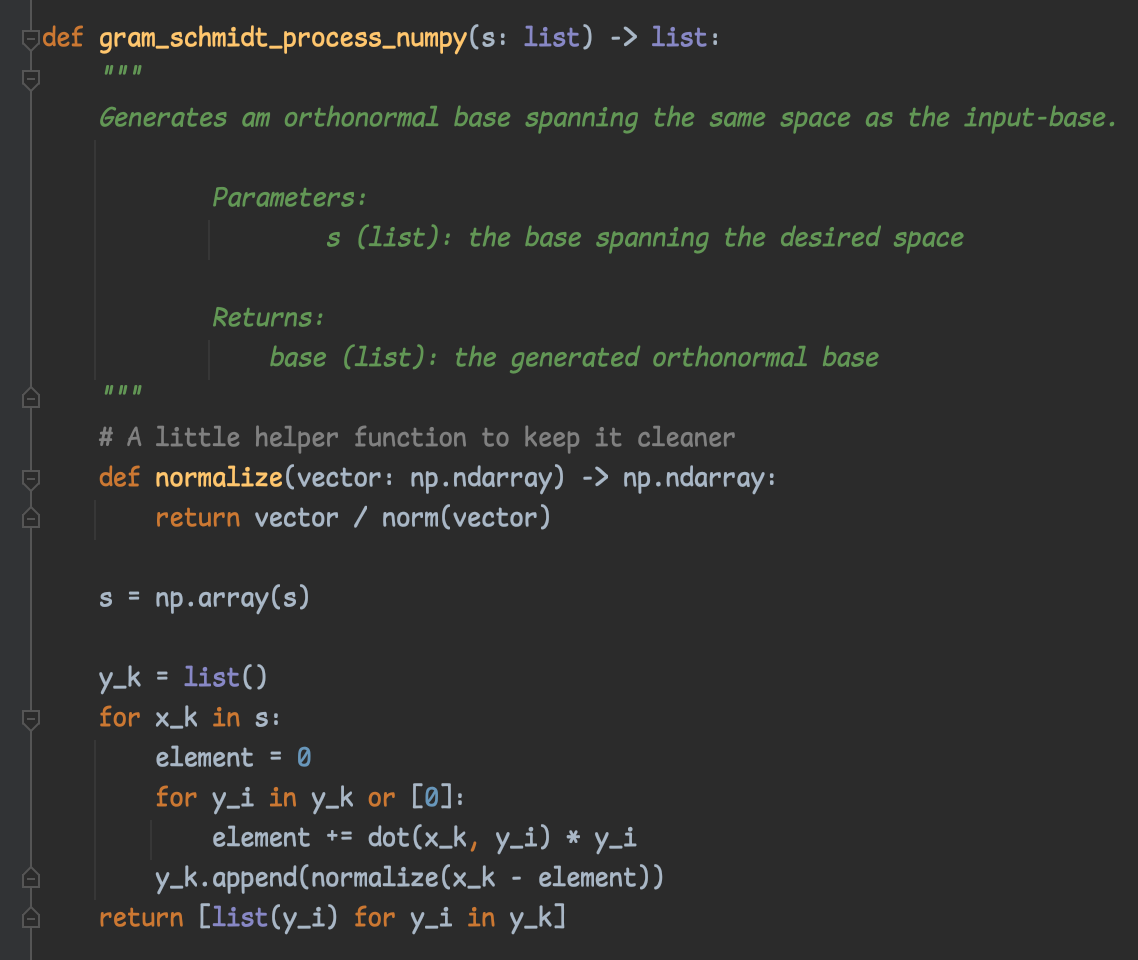
\includegraphics[width=7.5cm]{code_numpy.png}
            \caption{\label{fig:blue_rectangle} code utilizing numpy}
        \end{figure}
    \end{minipage} \hfill
    \begin{minipage}{0.35\textwidth}
        \tiny
        The most difficult part for me was input handling. Numpy provides such vast functionality that implementing the actual algorithm was rather easy.\\
        Implementing the manual version was trickier, as it was necessary to define the various functionalities manually. It might be easier to work with classes, but I decided to not use OOP at all. The manual implementation of the operations allows us to use the same code for the Gram-Schmidt process with different definitions of operations such as inner product.\\
        For more detail see the python files accompanying this presentation.
    \end{minipage}
\end{frame}

%---------------------------------------------------------
\begin{frame}{Recommended Literature}
    \begin{itemize}
    	\item Basic Linear Algebra, Blyth, T.S. and Robertson, E.F., 2002, Chapter 5
    	\item Further Linear Algebra, Blyth, T.S. and Robertson, E.F., 2002, Chapter 1
    	\item Math for AI 1-3 manuscript from WS19-WS20, Ullrich M., 2021, Chapter 11
    	\item Essence of linear algebra (video series), Sanderson G. (3blue1brown), 2016, accessed 15.08.2022, \url{https://www.3blue1brown.com/topics/linear-algebra}, \url{https://youtube.com/playlist?list=PLZHQObOWTQDPD3MizzM2xVFitgF8hE_ab}
    \end{itemize}
\end{frame}

%---------------------------------------------------------
\begin{frame}
    Thank you for your attention!\\
    \vspace{10mm}
    Presentation made by Pascal Pilz, 12111234, \href{mailto:pasc.pilz@gmail.com}{pasc.pilz@gmail.com}, for the course "KO Mathematics for AI II", 324.813, by Jan-Michael Holzinger, at Johannes Kepler University Linz.\\ \vspace{10mm}
    For the code implementation see \url{https://github.com/pilzpascal/KO_Mathematics_for_AI_II}
\end{frame}

\end{document}